\chapter{User Interface Design and Implementation}
\section{Finilized Product}
Here, we reflect on the changes that were ultimitly made to simplify our design.
\subsection{Pages for a visitor}
When a user first comes to see our website, they will be greeted with this page:
\begin{figure}[H]
\centering
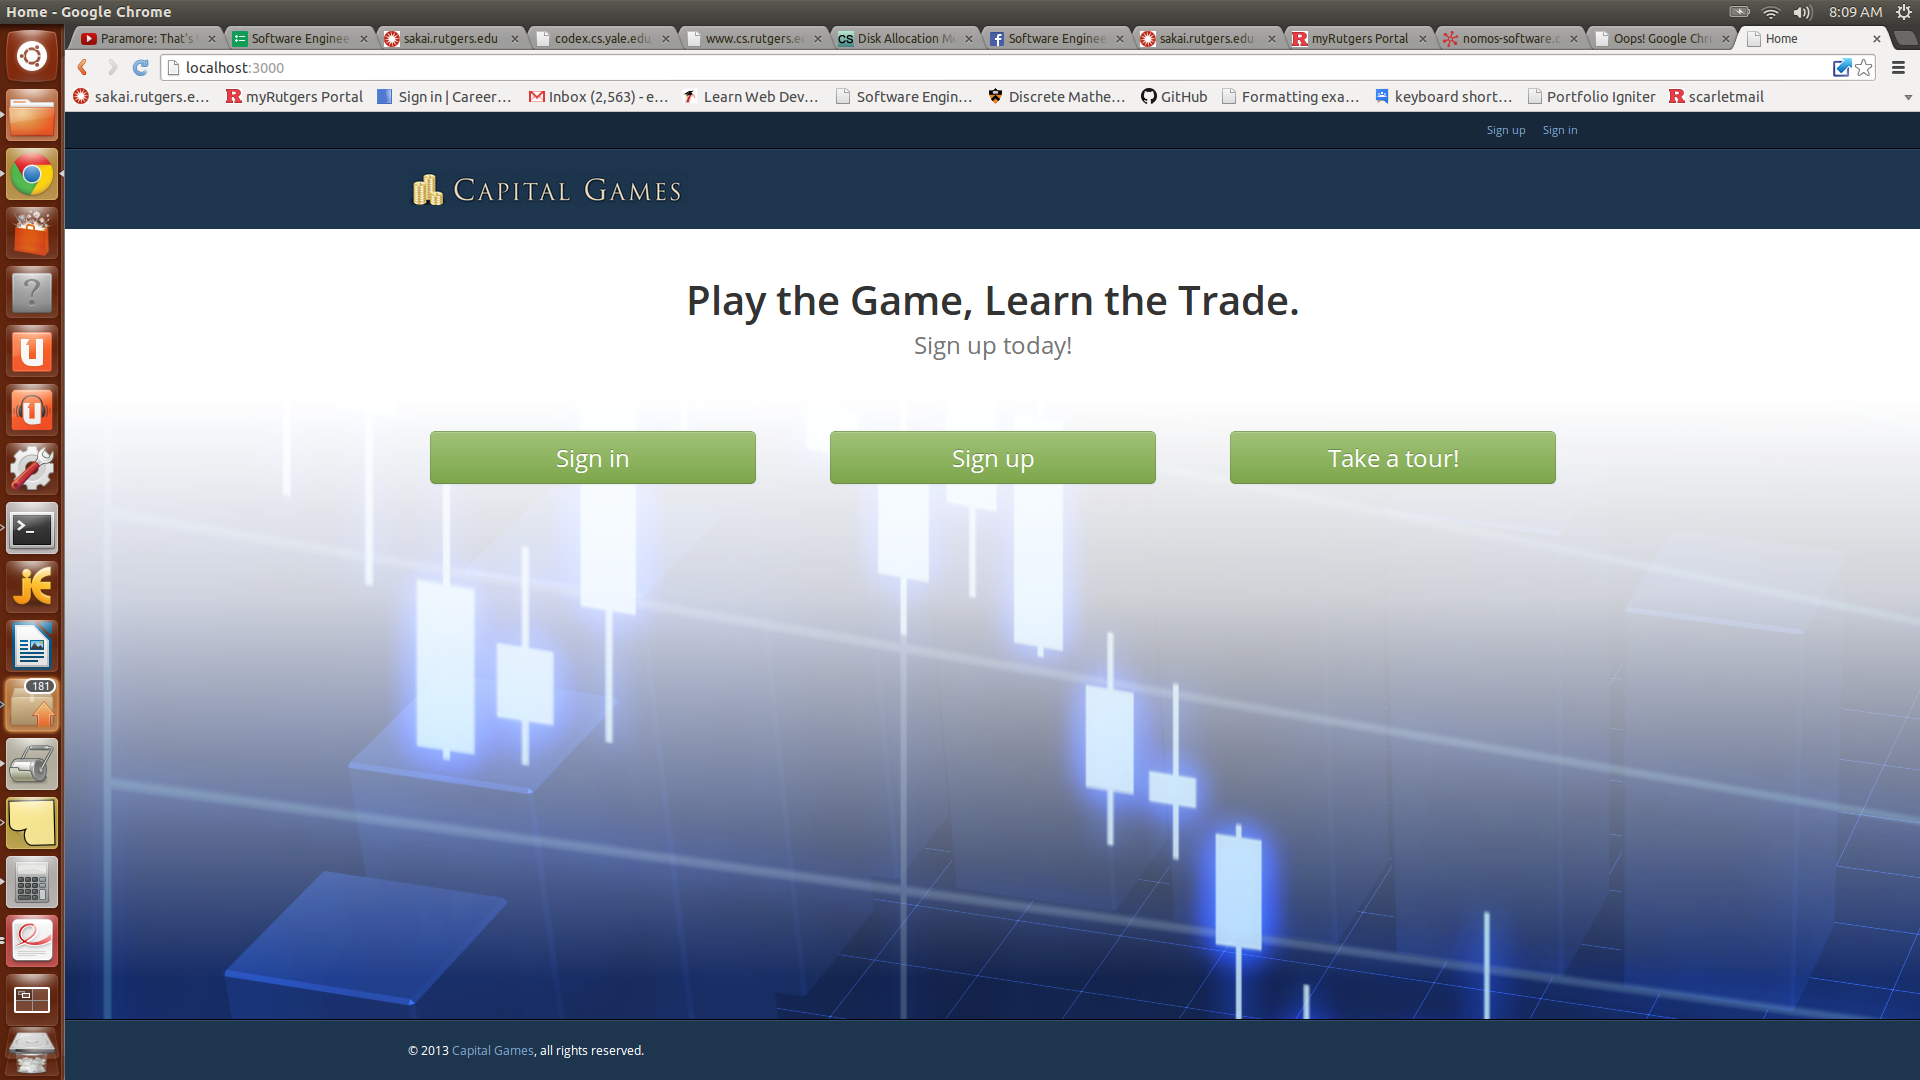
\includegraphics[width=5.5in]{./img/finalDesign/homepage.png}
\caption{Homepage of the website}
\end{figure}
If they click on the sign-in option, they will be taken to this page:
\begin{figure}[H]
\centering
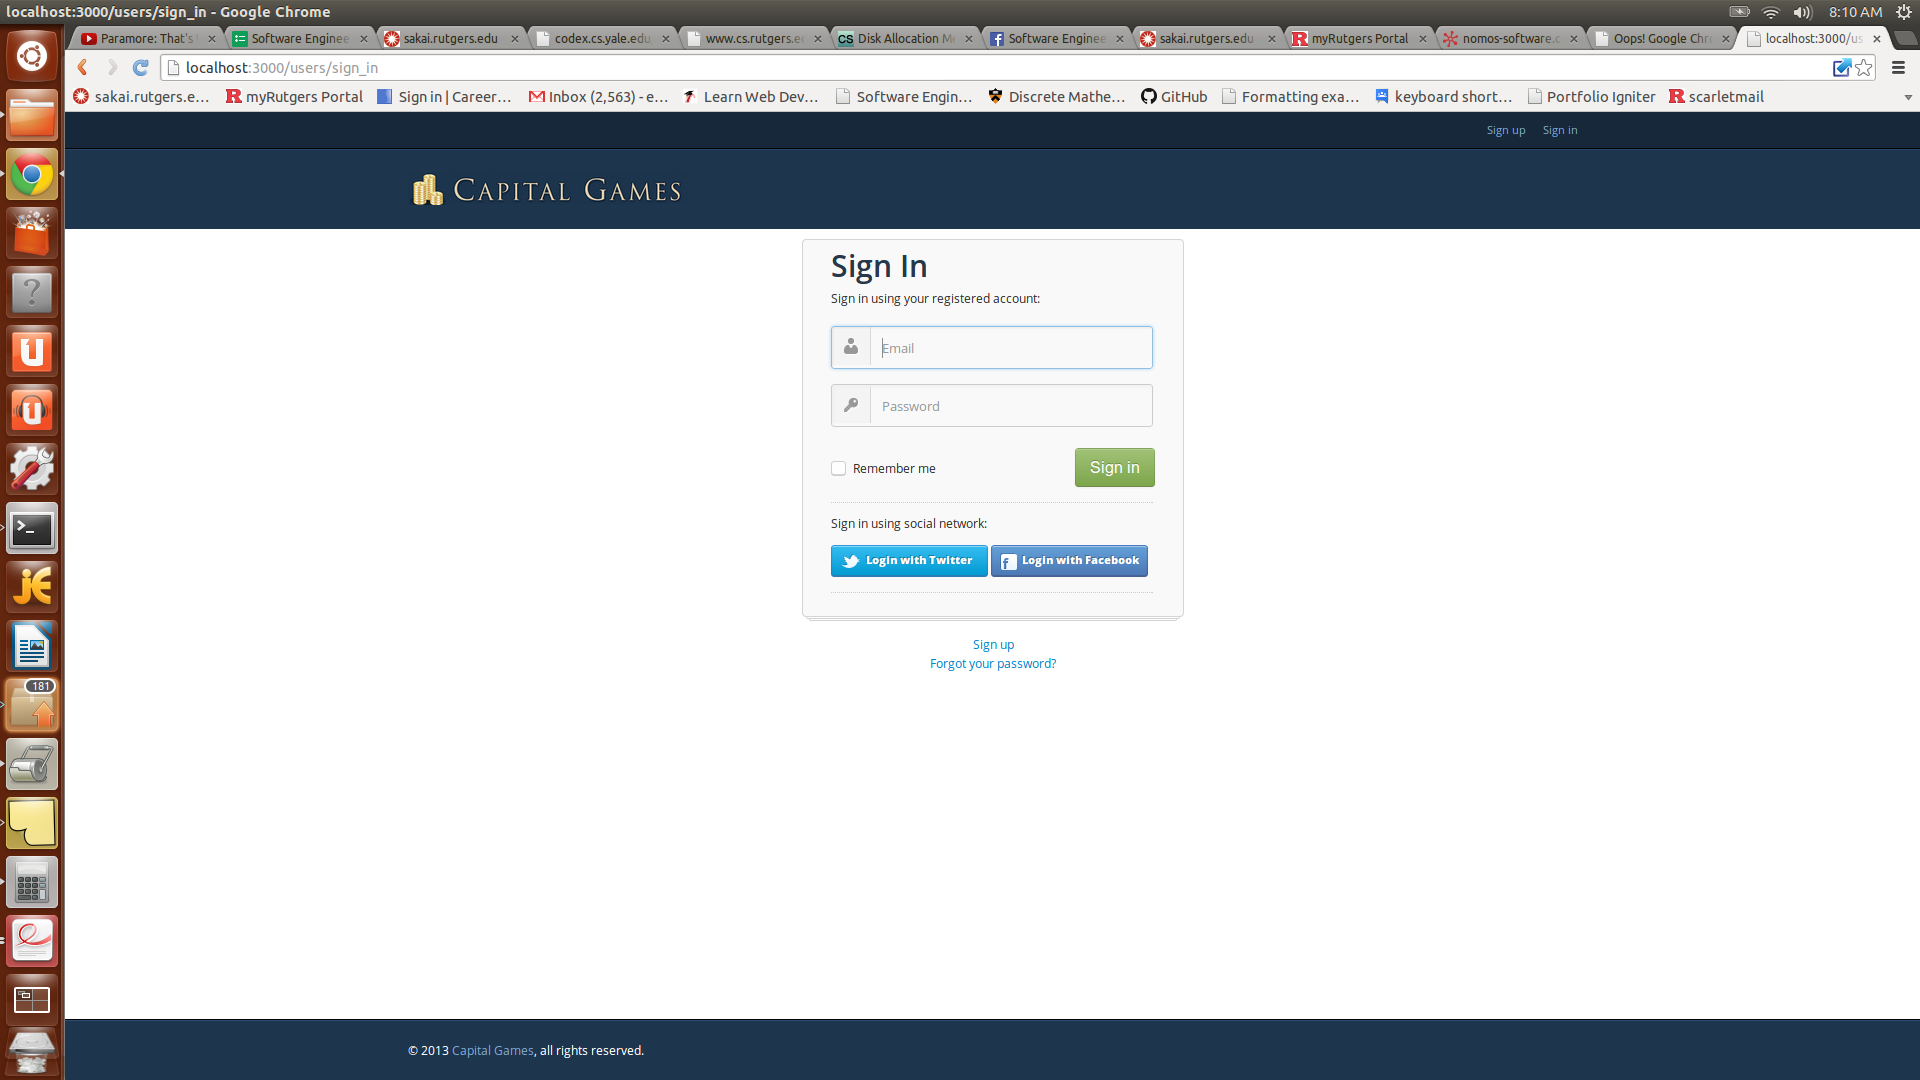
\includegraphics[width=5.5in]{./img/finalDesign/login.png}
\caption{The login page}
\end{figure}
Alternatively, if they click on the sign-up page, they wil be greeted with this page:
\begin{figure}[H]
\centering
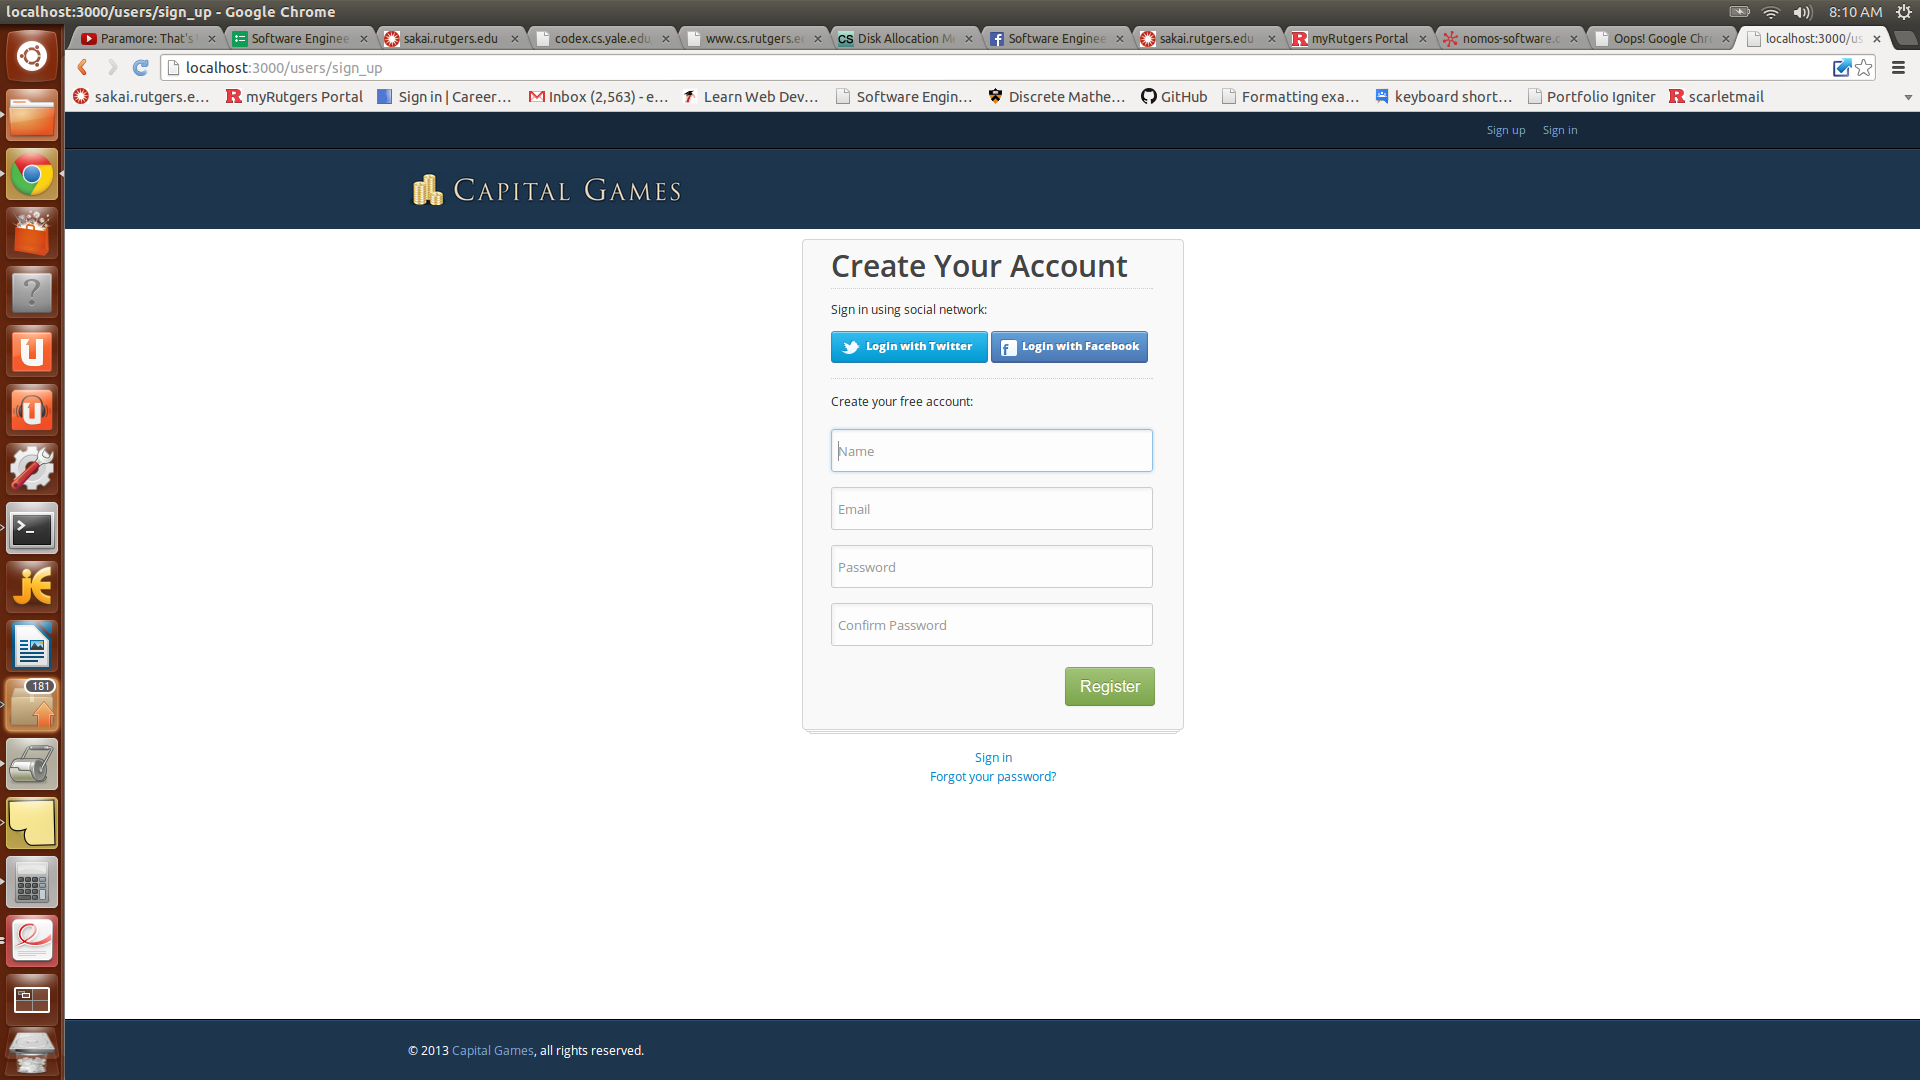
\includegraphics[width=5.5in]{./img/finalDesign/signup.png}
\caption{The sign-up page}
\end{figure}
Lastly, if they click on the "Take a Tour" button, they will be taken to our "Learn" section of the website. It's a simple text guided tour through our website that lets the user learn a little bit about the way our site works before (or after) signing up.
\begin{figure}[H]
\centering
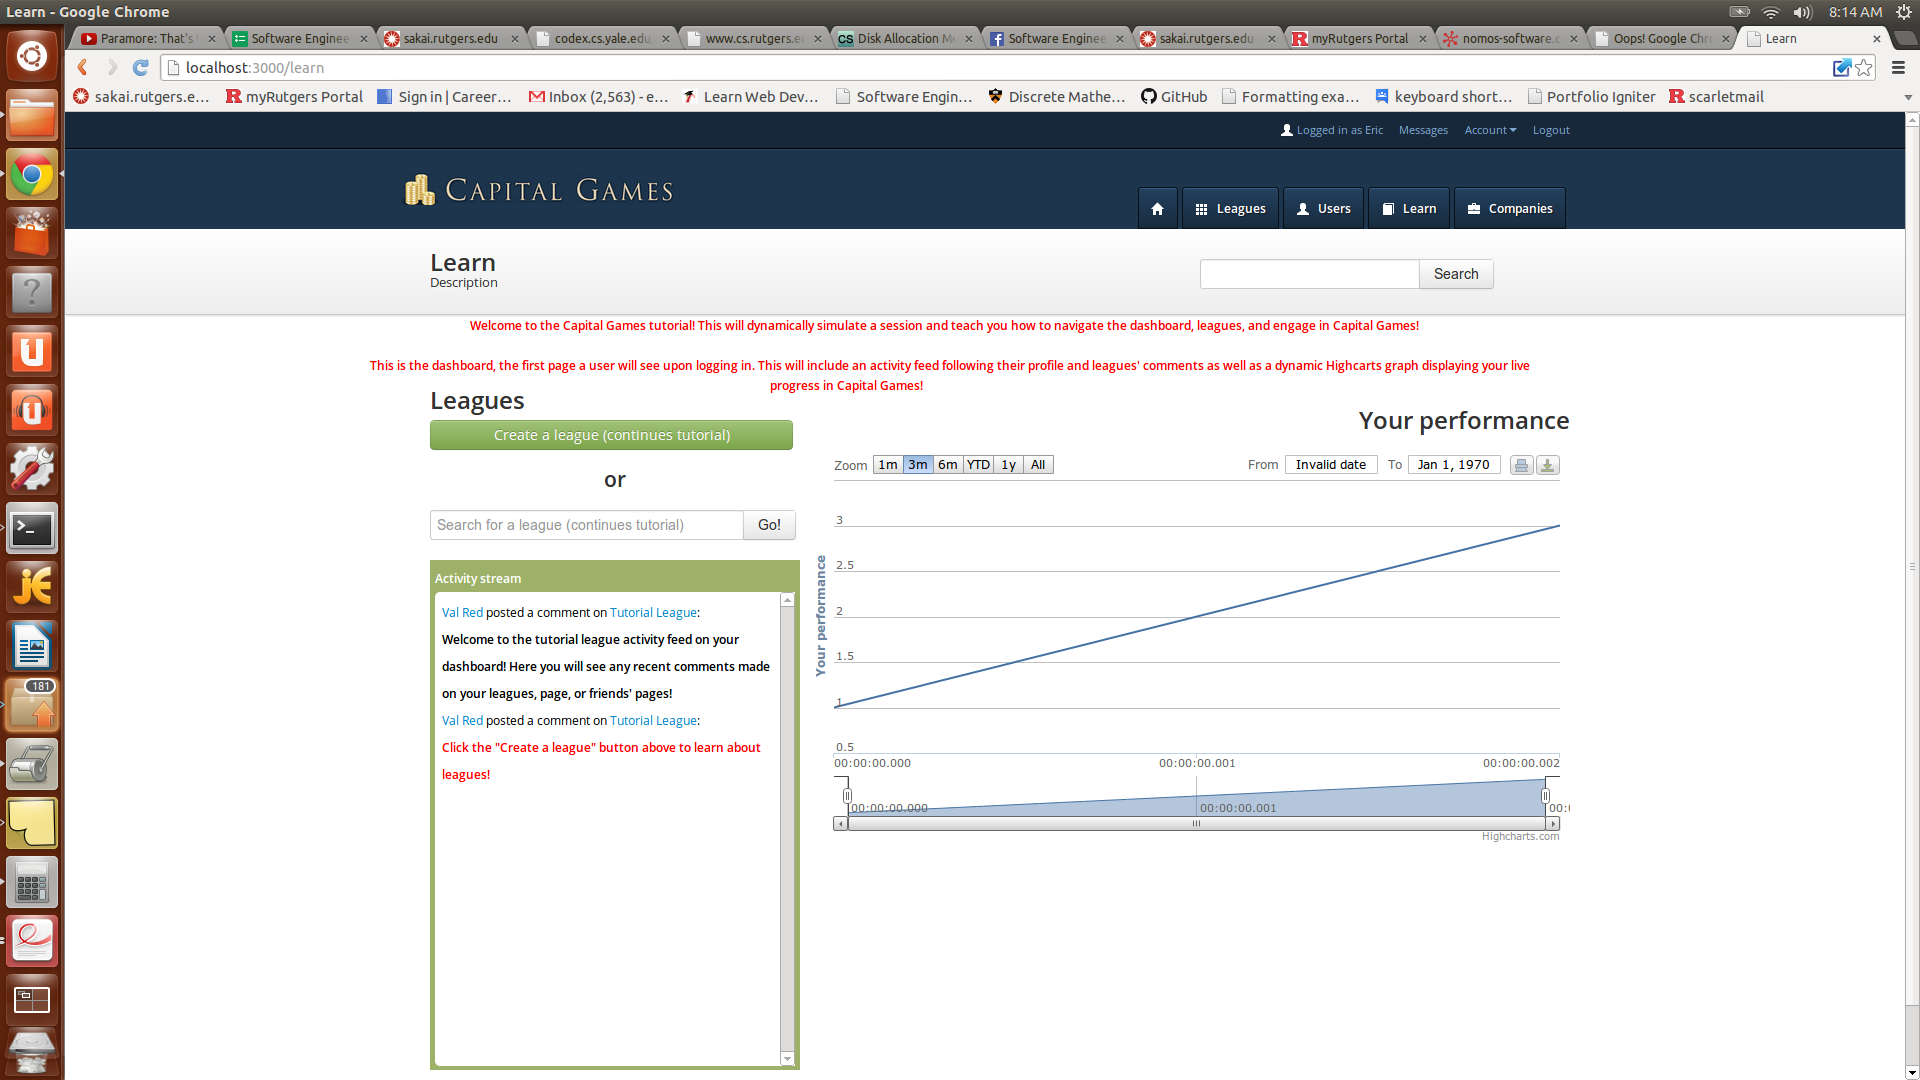
\includegraphics[width=5.5in]{./img/finalDesign/tutorial.png}
\caption{The first tutorial}
\end{figure}
\subsection{The Dashboard}
Once a user is logged in, they will be greeted with their dashboard. This is a customized page that thells them information about some events that have been going on in the site as well as the progress in all of thier leagues.
\begin{figure}[H]
\centering
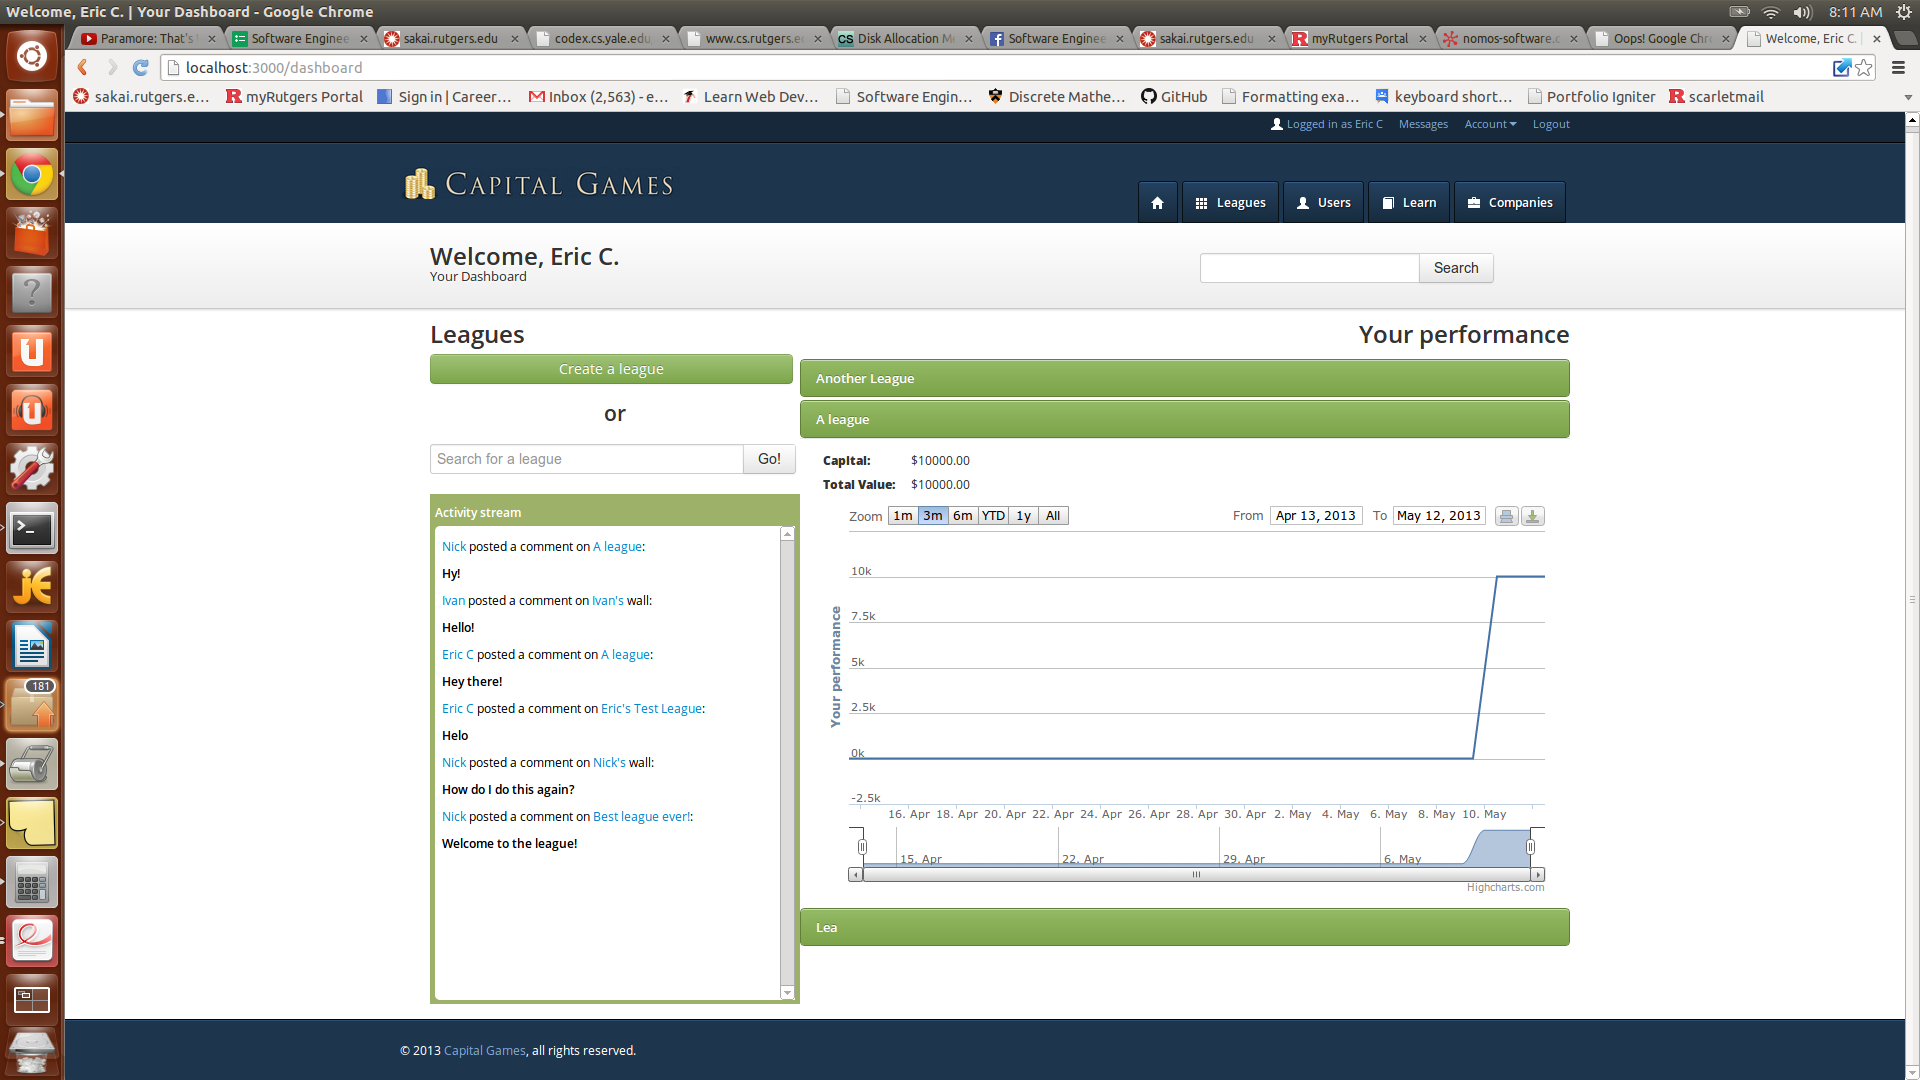
\includegraphics[width=5.5in]{./img/finalDesign/dashboard.png}
\caption{The Dashboard}
\end{figure}
\subsection{Leagues}
The final design for leagues was simplified the most. If you want to find a league, you visit the leagues page. There you can search, filter through, or create a league. 
\begin{figure}[H]
\centering
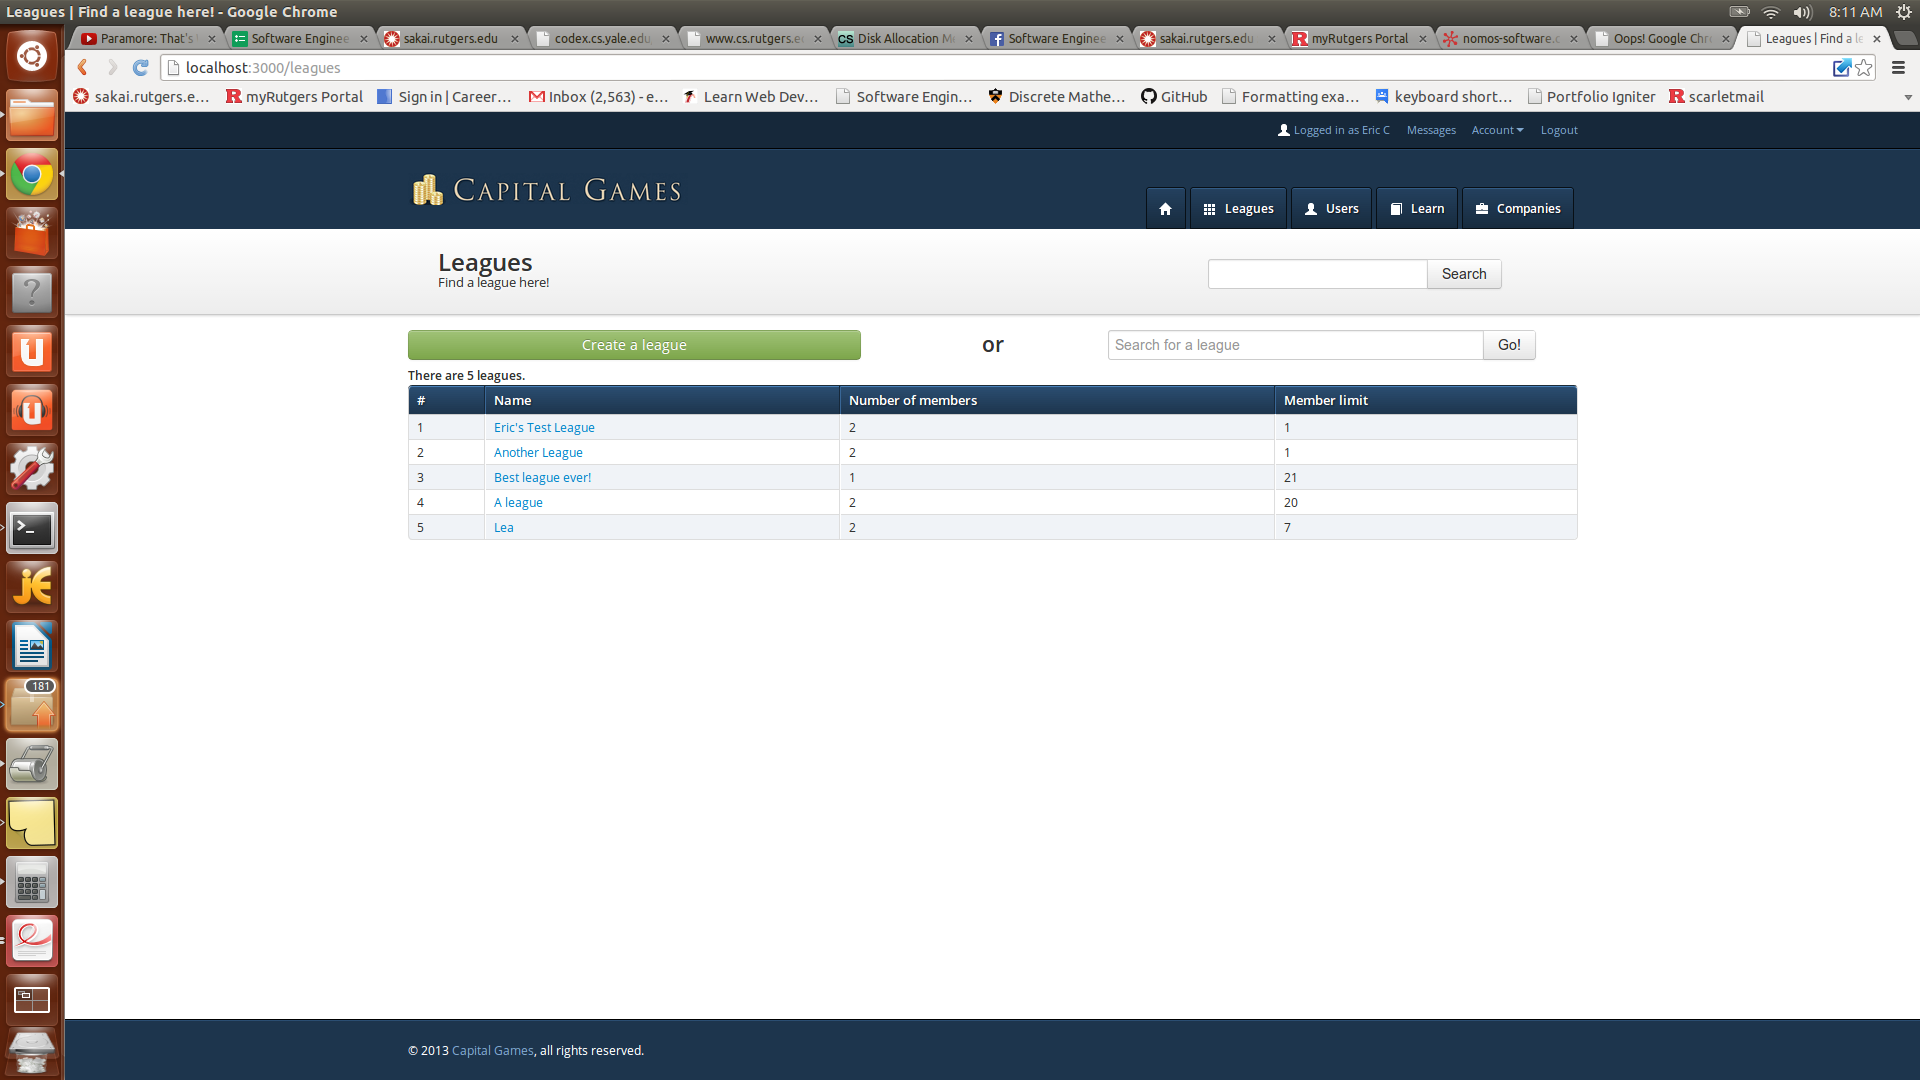
\includegraphics[width=5.5in]{./img/finalDesign/leagues.png}
\caption{The leagues page}
\end{figure}
If you want to create a league, you will be greeted with a very simple page for making a league.
\begin{figure}[H]
\centering
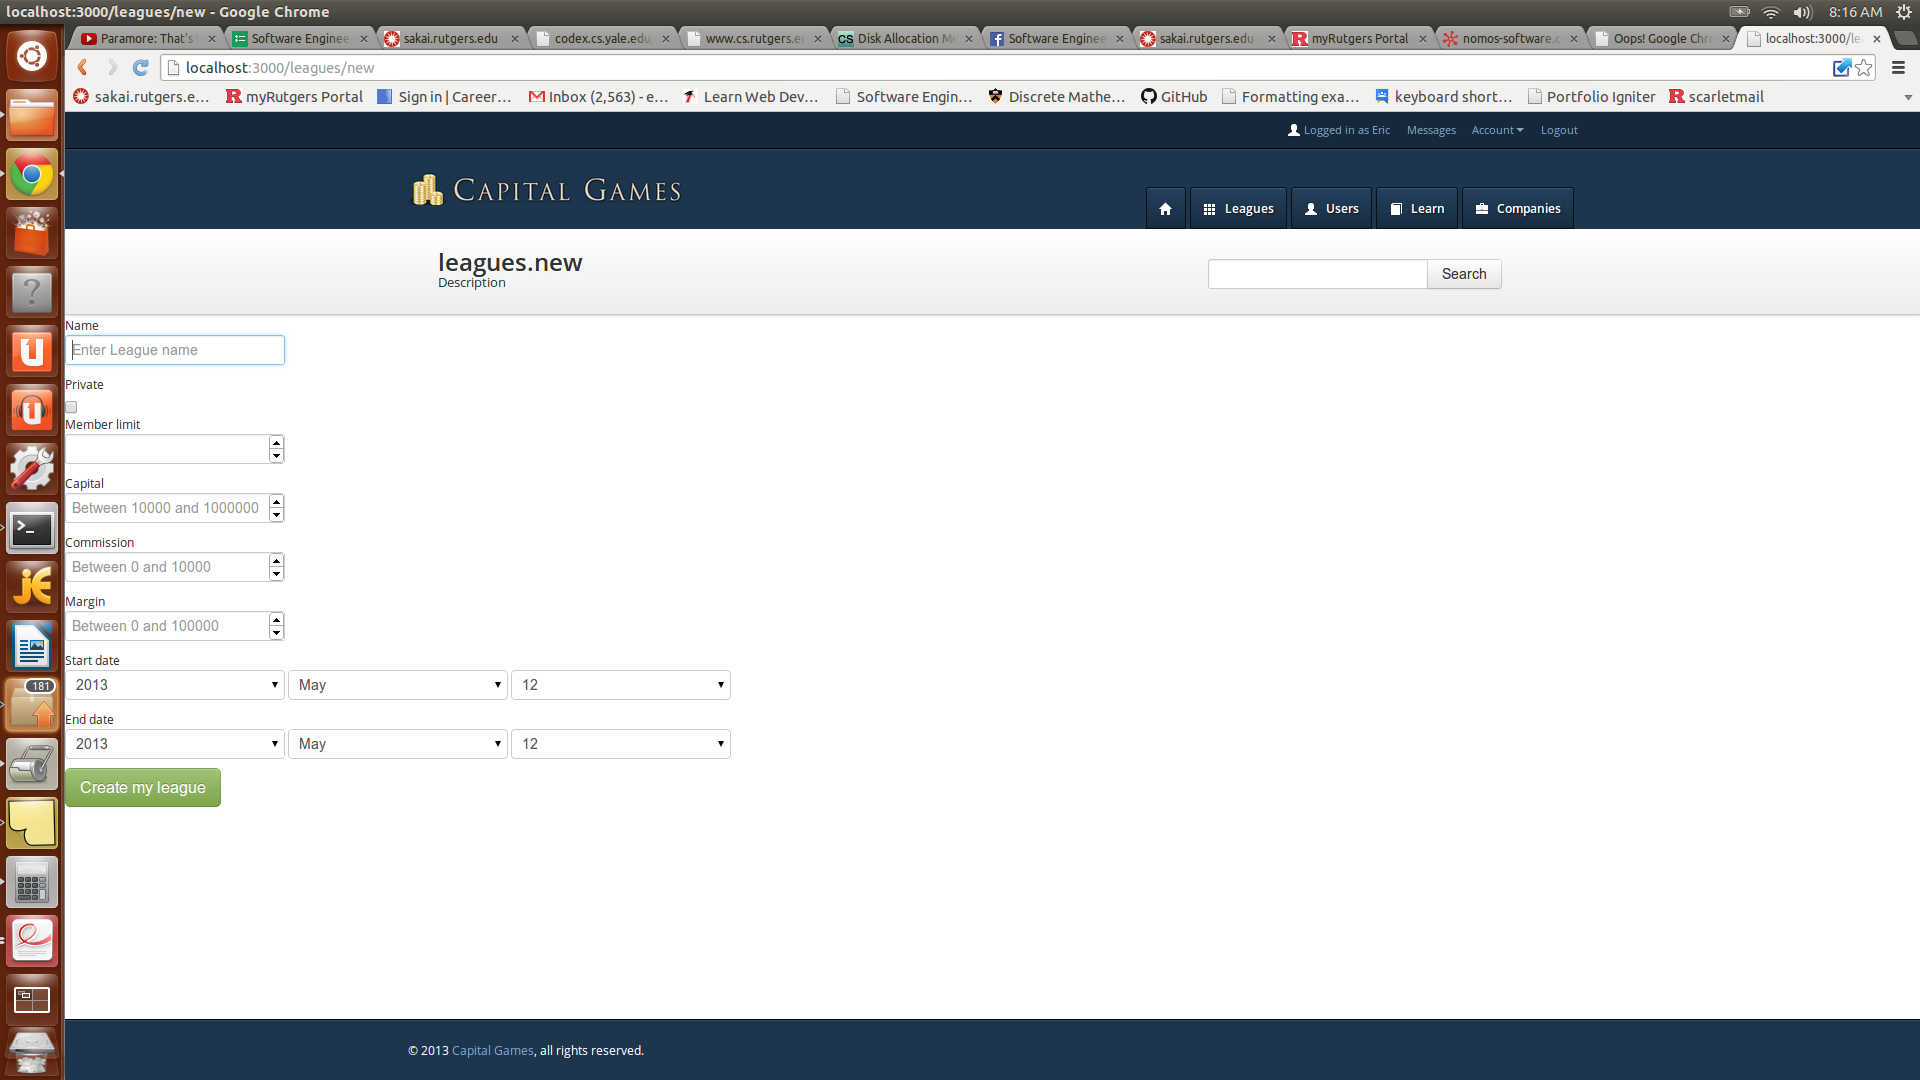
\includegraphics[width=5.5in]{./img/finalDesign/createleague.png}
\caption{The create a league page}
\end{figure}
Once you have a league or are in it, you can check out how users are doing by checking out the table with users sorted by their rank or see comments that other users have posted.
\begin{figure}[H]
\centering
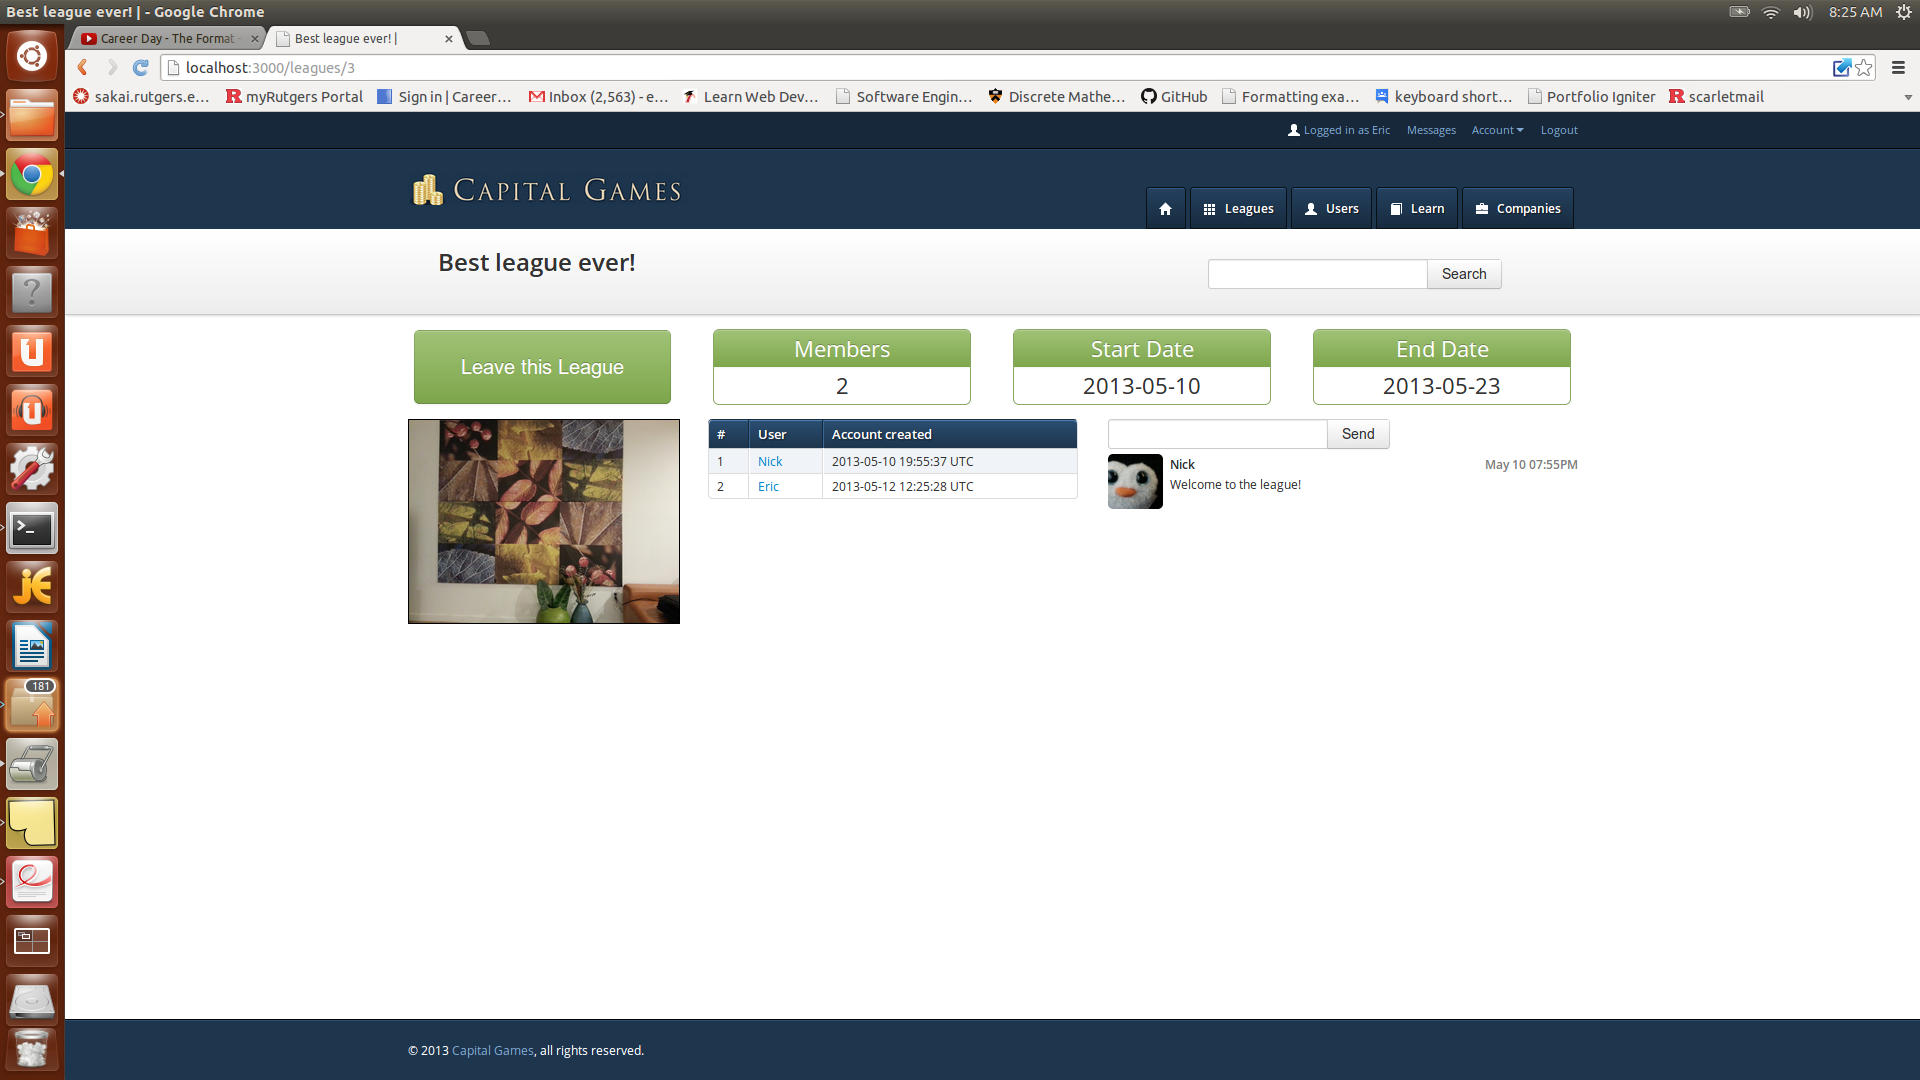
\includegraphics[width=5.5in]{./img/finalDesign/league.png}
\caption{A league page}
\end{figure}
If you're an admin of the page, you can check out the league settings, where you can change the name, description and league picture in the "Basic Settings" tab, and you can delete the league in the "Delete League" tab. The others were not implemented yet.
\begin{figure}[H]
\centering
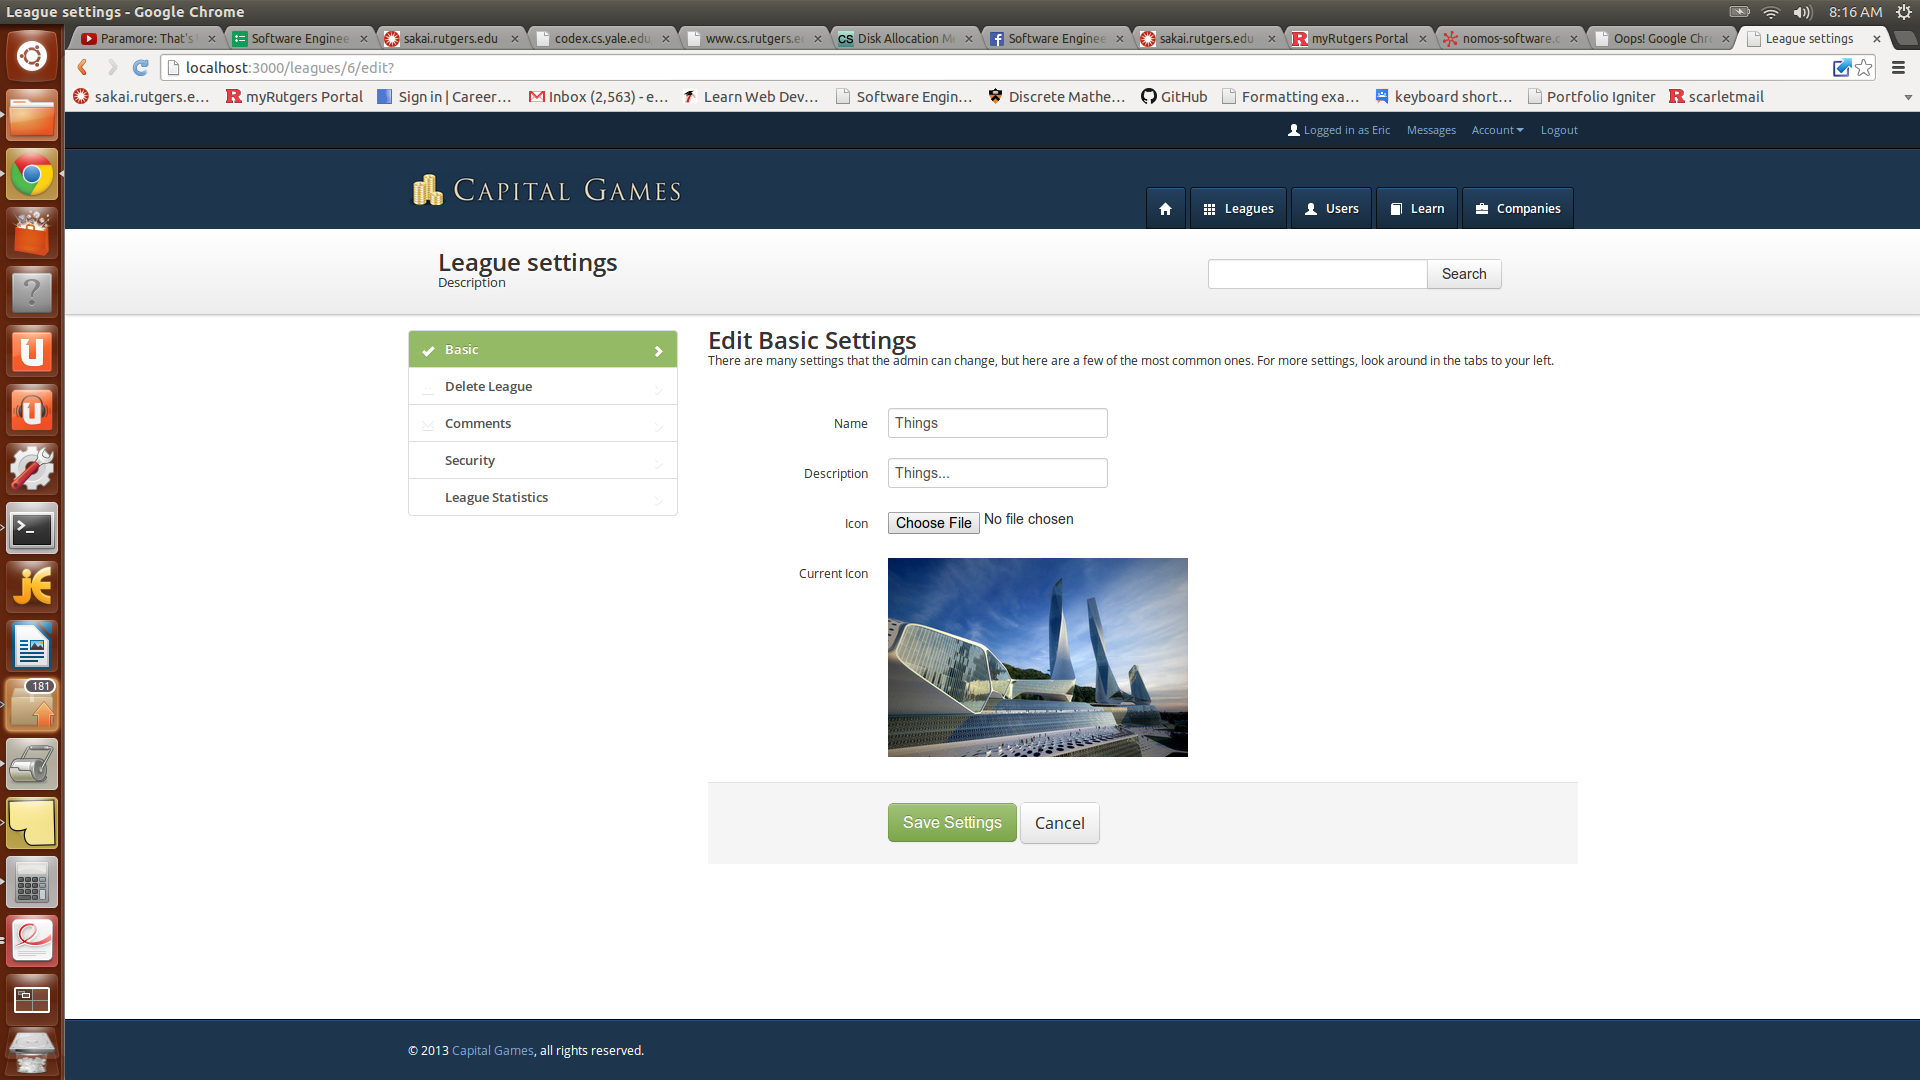
\includegraphics[width=5.5in]{./img/finalDesign/leaguesettings.png}
\caption{The league settings page}
\end{figure}
If you want to check out a user's performance in the league, you just have to click on their name on the table in the league page. Here, you can see their rank, worth, and recent orders they have made.
\begin{figure}[H]
\centering
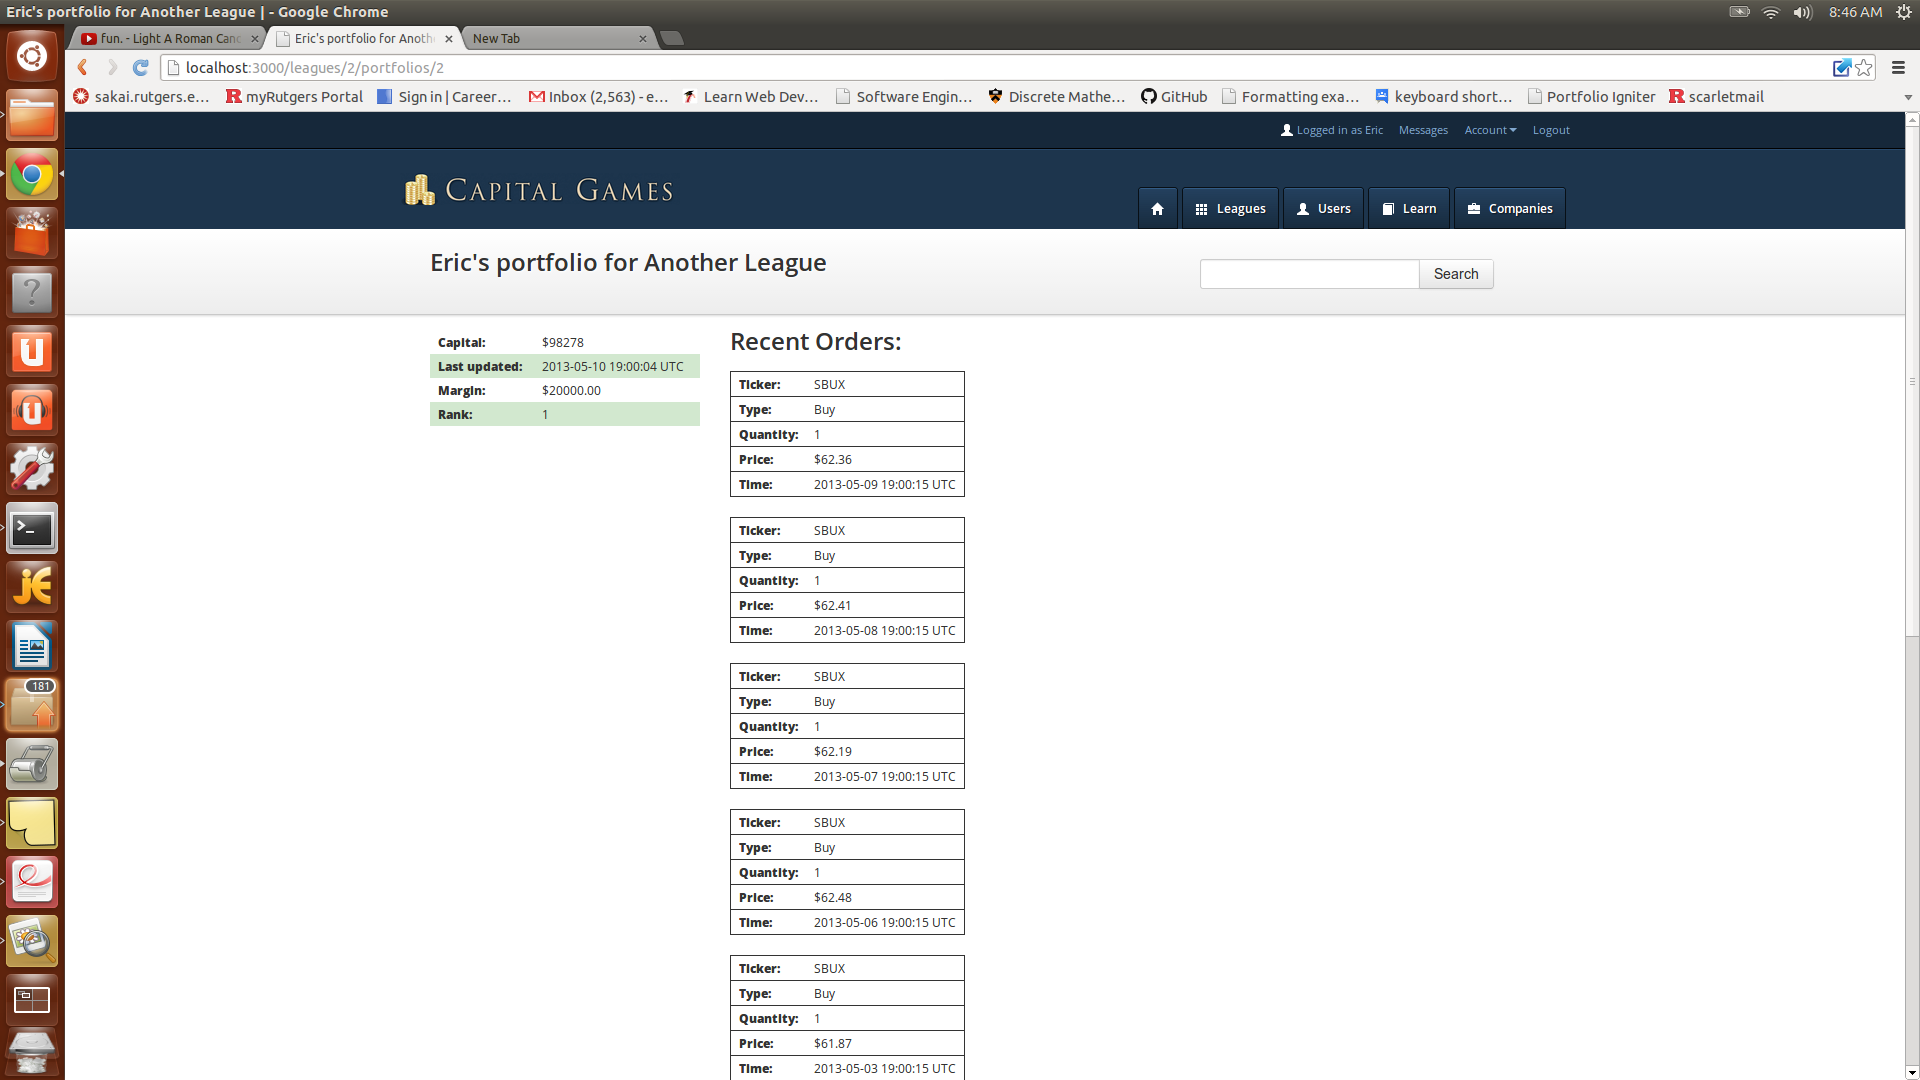
\includegraphics[width=5.5in]{./img/finalDesign/port.png}
\caption{The portfolio page}
\end{figure}
\subsection{Users}
With our specialized social system, it's easy to keep in touch with other users. One way you can do that is by dropping a comment on their wall. Their wall is a place that displays their profile picture, their leagues and their comments. 
\begin{figure}[H]
\centering
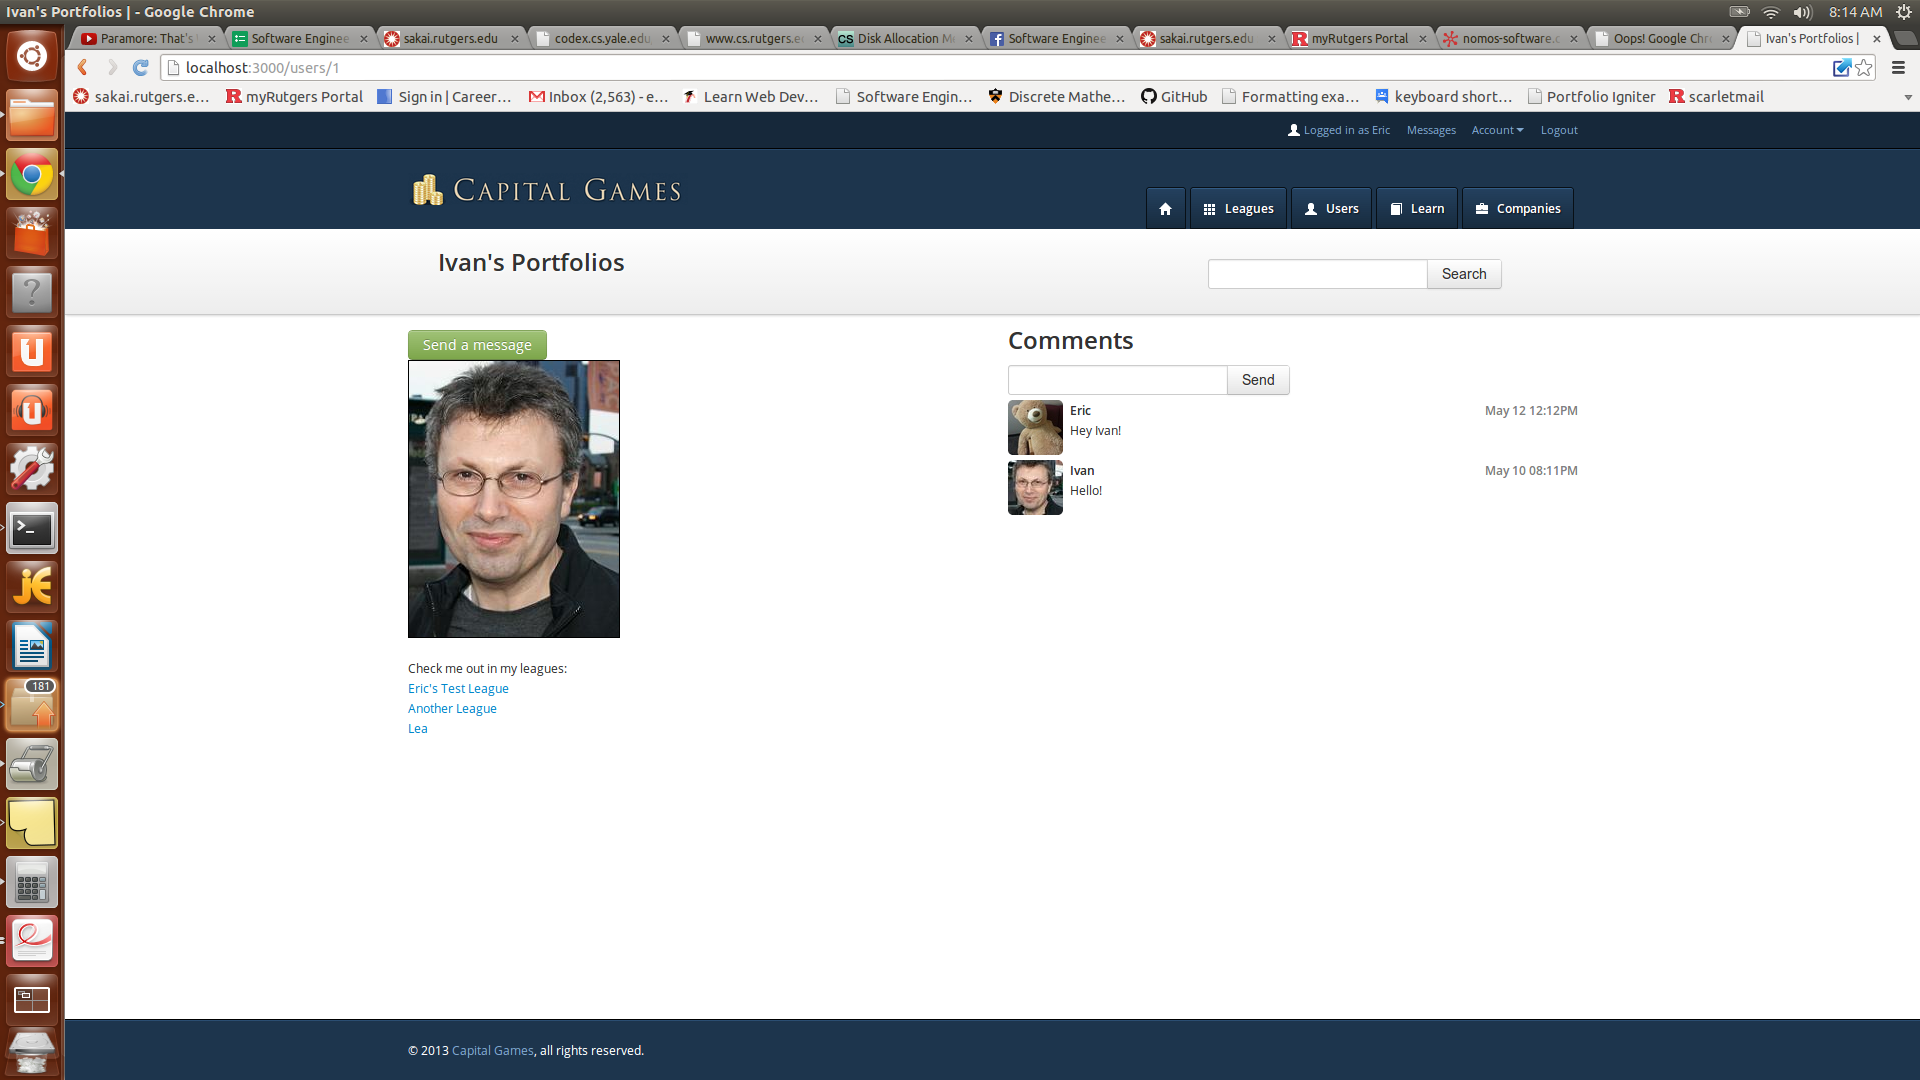
\includegraphics[width=5.5in]{./img/finalDesign/user.png}
\caption{The user page}
\end{figure}
If one wants to change their settings, they can look up at the top bar in the header and click on "Account" and then "Settings". This will allow you to change your name and your profile picture.
\begin{figure}[H]
\centering
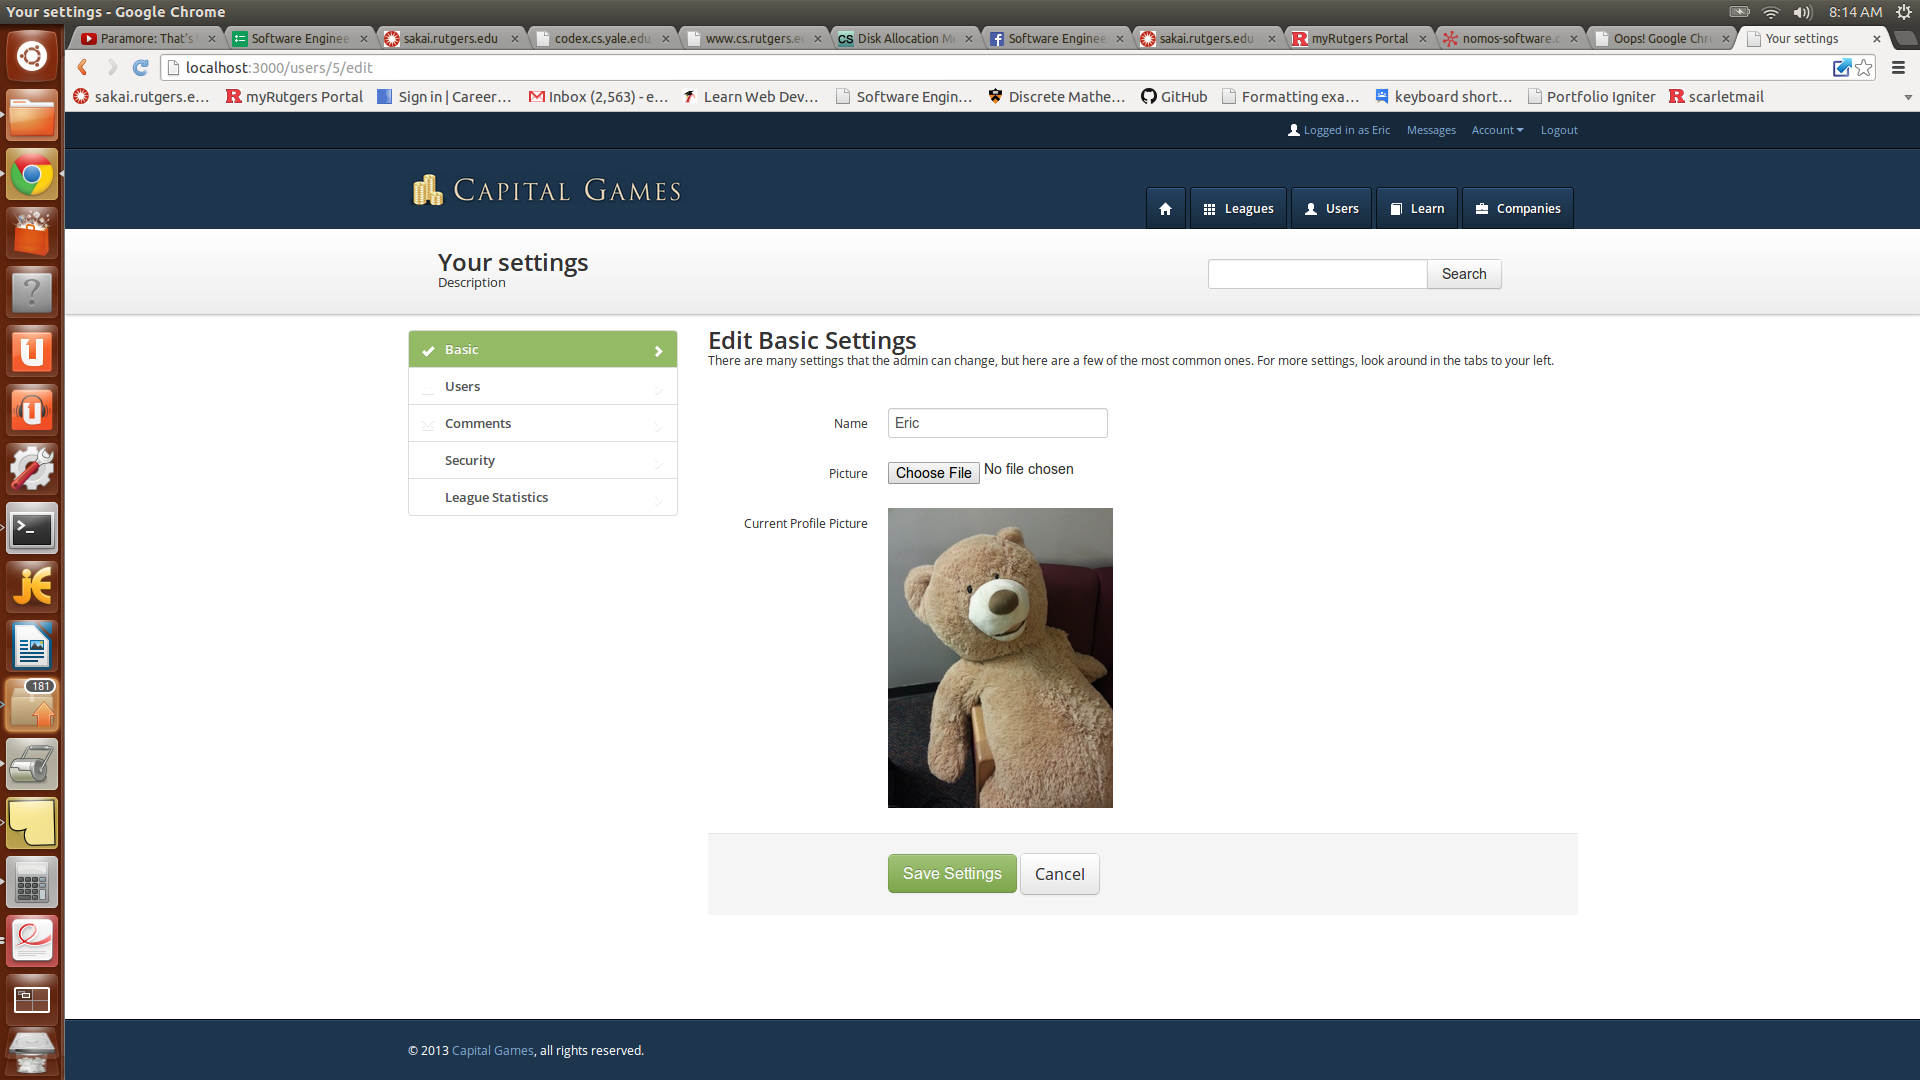
\includegraphics[width=5.5in]{./img/finalDesign/usersettings.png}
\caption{The user settings page}
\end{figure}
\subsection{Companies}
The last part of the website that we will highlight is the companies pages. You can go to the "Companies" page of the website and you will be greeted with recent news about the market and the ability to search for a company by symbol. 
\begin{figure}[H]
\centering
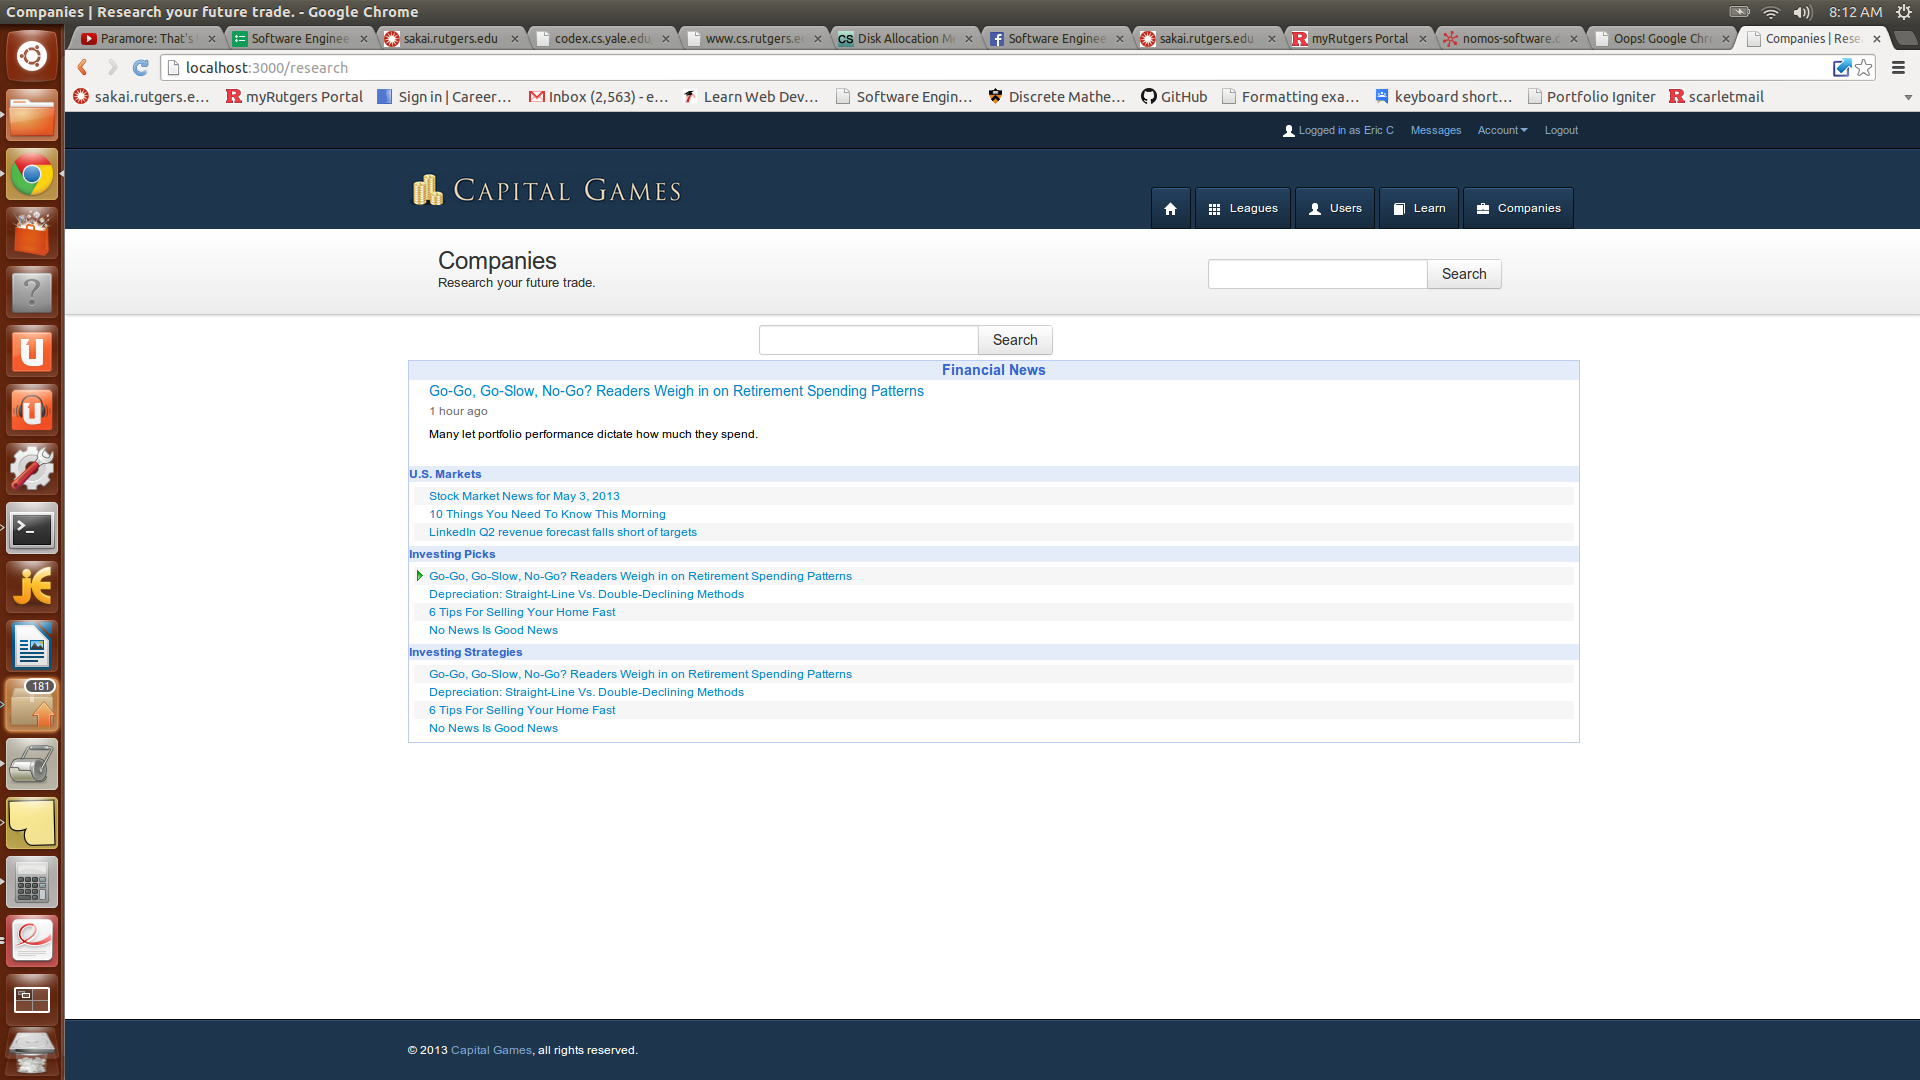
\includegraphics[width=5.5in]{./img/finalDesign/companies.png}
\caption{The companies page}
\end{figure}
Once you search for a company, you will find a lot of relevant information about that company to help you in your purchase of stocks. 
\begin{figure}[H]
\centering
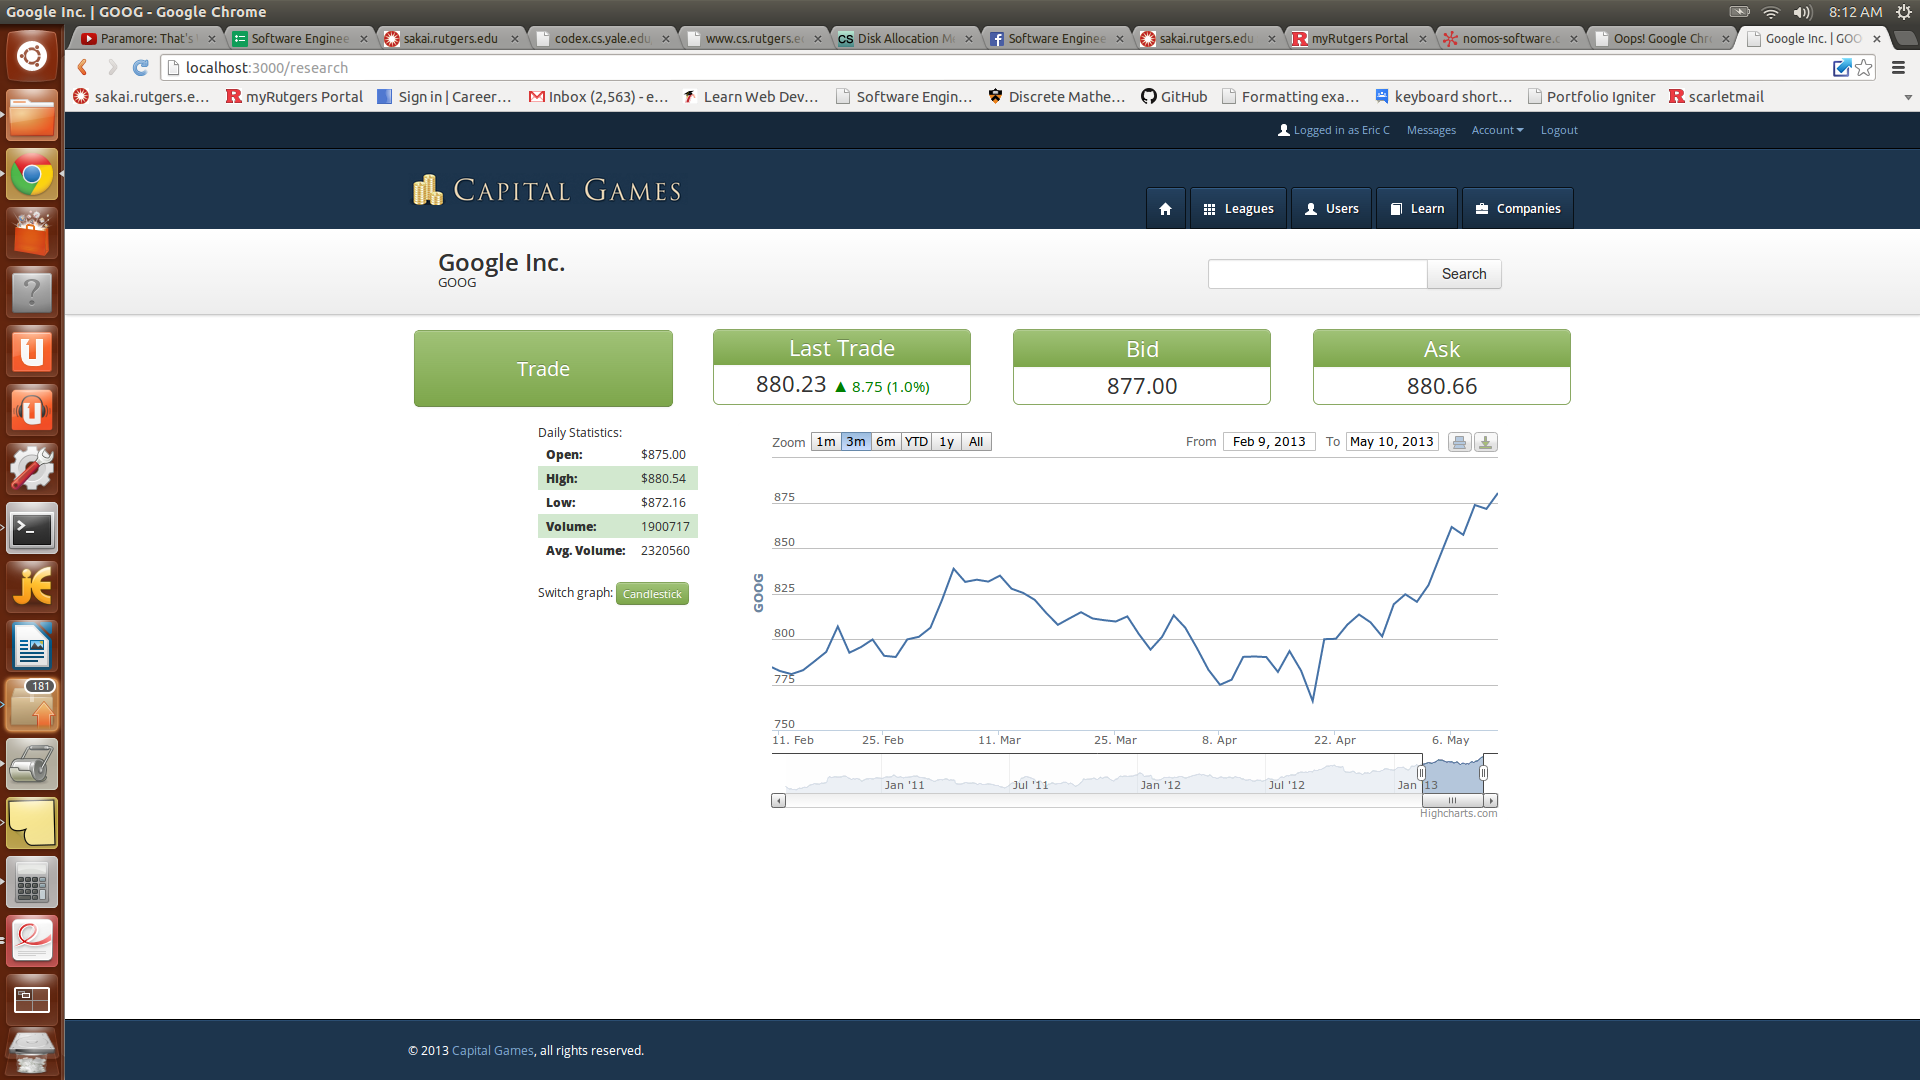
\includegraphics[width=5.5in]{./img/finalDesign/company.png}
\caption{A company page}
\end{figure}
If you want to buy/sell a stock, you can press on the "Trade" button, which bring up this dialogue:
\begin{figure}[H]
\centering
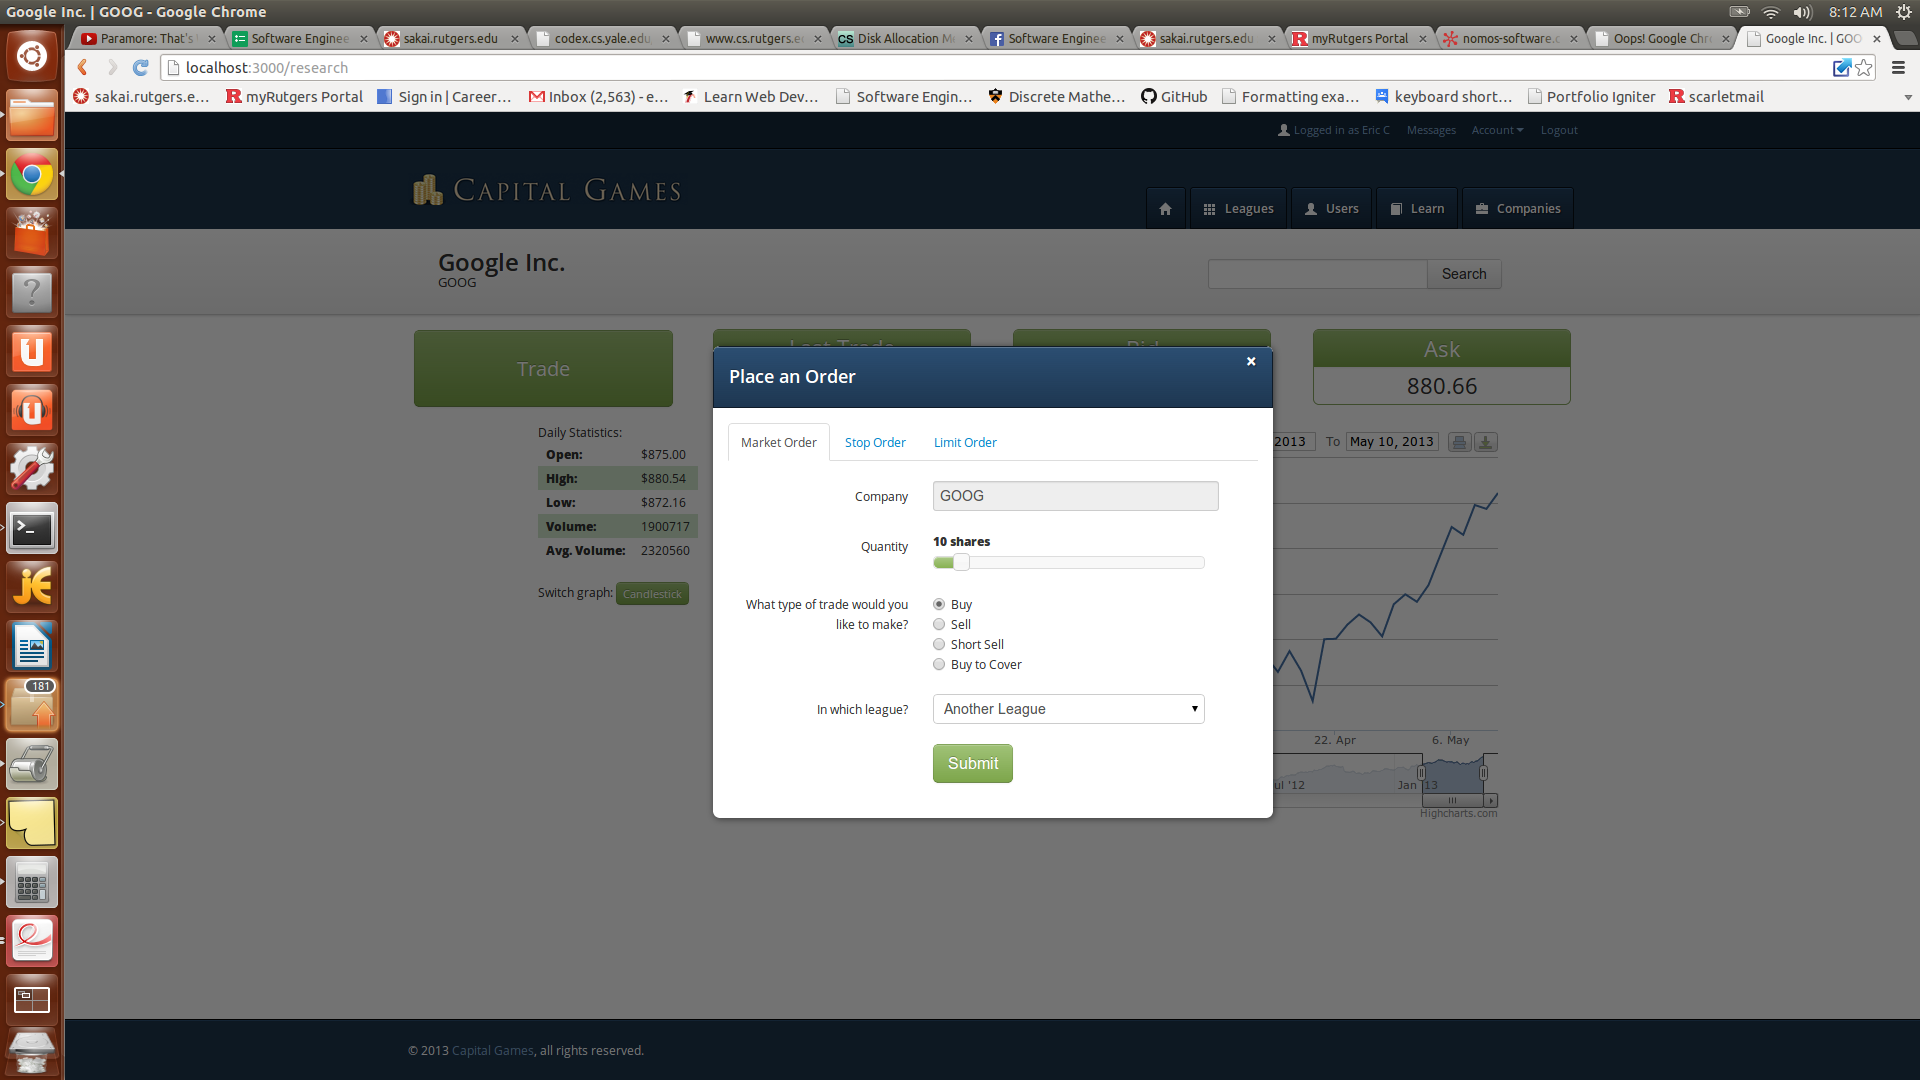
\includegraphics[width=5.5in]{./img/finalDesign/buy.png}
\caption{Buying or selling stocks}
\end{figure}
There are a lot of options to choose from there and they all work as the usual market does.
